%!tex root = ../main.tex

%\section{Automatically proving lower bounds for LCL problems} \label{sec:implementation}
\section{Implementation} \label{sec:implementation}
In this section, we will explain all the modules that we use in the implementation of the Algorithm~\ref{alg:counterexample_finder}.
The implementation itself is a computer program~\cite{NonconstantLclClassifier2022}, that attempts to automatically find a proof of unsolvability for an LCL problem in the PN model.
Although we have used Rust programming language~\cite{RustLang} for the implementation, we keep the explanations independent of any programming language.

%This includes the previously declared functions $\textsc{SolutionExists}(\Pi, g)$ and $\textsc{GenerateGraphs}(n, \Delta, \delta)$, which were given as black boxes.
In Section~\ref{sec:implementation:generating_multigraphs}, we discuss how we generate multigraphs, and describe the function $\textsc{GenerateGraphs}(n, \Delta, \delta)$.
In Section~\ref{sec:implementation:sat}, we discuss Boolean satisfiability problems (SAT), and in Section~\ref{sec:implementation:our_sat}, we discuss how we use SAT to implement the function $\textsc{SolutionExists}(\Pi, g)$.
As we are interested in classifying not just one LCL problem, but a class of problems, we need to know how to generate them.
In Section~\ref{sec:implementation:generating_lcl_problems}, we discuss how we generate LCL problems.
Lastly, we discuss some optimizations in our implementation in Section \ref{sec:implementation:optimizations}.


\subsection{Generating Multigraphs} \label{sec:implementation:generating_multigraphs}
A naive way to generate $(\Delta, \delta)$-biregular multigraphs is to generate all possible multigraphs, and then filtering out graphs that are not in the graph family.
Note that there are \(2^{\frac{n(n-1)}{2}}\) different simple graphs of size $n$.
The number of simple graphs grows exponentially fast, as shown in Table~\ref{tbl:graph_count_growth}.
Generating all graphs of size $n$ may take forever on modern computers even for small values of $n$.
%0, 1, 3, 6, 10, 15, 21, 28, 36, 45, 55,
%1, 2, 8, 64, 1024, 32768, 2097152, 268435456, 68719476736, 35184372088832, 36028797018963968
\begin{table}[H]
  \centering
  \begin{tabular}{r|rr}
    \toprule
    $n$&Edges&Graphs\\
    \midrule
    1 & 0 &1\\
    2 & 1 &2\\
    3 & 3 &8\\
    4 & 6 &64\\
    5 & 10 &1024\\
    6 & 15 &32768\\
    7 & 21 &2097152\\
    8 & 28 &268435456\\
    9 & 36 &68719476736\\
    10 & 45 &35184372088832\\
    11 & 55 &36028797018963968\\
    \vdots & \vdots &\vdots\\
    \bottomrule
  \end{tabular}
  \caption{
    A list of number of edges in complete graphs, and the number of simple graphs.
  }
  \label{tbl:graph_count_growth}
\end{table}

In this experiment we did not even consider multiple edges.
With multiple edges without any limits, the number of multigraphs is infinite.
However, this is not true when we consider only $(\Delta, \delta)$-biregular multigraphs of size $n$.
Clearly the number of multiple edges is bounded by $\max(\Delta, \delta)$.

We call the parts of a biregular graph as $A$ and $B$ (see Section~\ref{sec:graphs}).
The numbers of incident edges for nodes of parts $A$ and $B$ are $\Delta$ and $\delta$, respectively.
There are only $n-1$ possibilities for pair $(|A|, |B|)$:
$$(1, n-1), (2, n-2), ..., (n-2, 2), (n-1, 1).$$
We know from Equation~\ref{eq:biregular:sum_of_degrees} that the sums of degrees of each node in each part must be equal.
Therefore, we need to consider only pairs $(n_A, n_B)$ such that the following hold
\begin{equation} \label{eq:pairs:1}
  \Delta n_A = \delta n_B,
\end{equation}
\begin{equation} \label{eq:pairs:2}
n_A + n_B = n.
\end{equation}
If we assume that $\Delta \geq \delta$, then we can see from Equation~\ref{eq:pairs:1} that $n_A\leq n_B$, therefore we only need to consider pairs

$$(1, n-1), (2, n-2), ..., (\left\lfloor\frac{n}{2}\right\rfloor, n - \left\lfloor\frac{n}{2}\right\rfloor).$$

For example with $(3,2)$-biregular multigraphs, we can only have the pair $(4, 6)$, as shown in Table~\ref{tbl:possible_pairs}.
However, most of the time there are no valid pairs for chosen $n$, as we can see for $n=9$ in Table \ref{tbl:possible_pairs:no_pairs}.

\begin{table}[H]
  \parbox{.45\linewidth}{
    \centering
    \begin{tabular}{rrrr}
    \toprule
    $n_A$&$n_B$&$\Delta n_A$&$\delta n_B$\\
    \midrule
    1 & 9 & 3  & 18\\
    2 & 8 & 6  & 16\\
    3 & 7 & 9  & 14\\
    \textbf{4} & \textbf{6} & \textbf{12} & \textbf{12}\\
    5 & 5 & 15 & 10\\
    \bottomrule
  \end{tabular}
  \caption{
    Possible pairs of node counts for part A and B in a $(3,2)$-biregular multigraph when $n=10$.
    The only valid pair with $\Delta n_A = \delta n_B$ is (4, 6), and it is bolded.
  }
  \label{tbl:possible_pairs}
  }
  \hfill
  \parbox{.45\linewidth}{
  \centering
  \begin{tabular}{rrrr}
    \toprule
    $n_A$&$n_B$&$\Delta n_A$&$\delta n_B$\\
    \midrule
    1 & 8 & 3  & 16\\
    2 & 7 & 6  & 14\\
    3 & 6 & 9  & 12\\
    4 & 5 & 12 & 10\\
    \bottomrule
  \end{tabular}
  \caption{
    Possible pairs of node counts for part A and B in a $(3,2)$-biregular multigraph when $n=9$.
    There are no valid pairs.
  }
  \label{tbl:possible_pairs:no_pairs}
  }
\end{table}

Equations~\ref{eq:pairs:1} and \ref{eq:pairs:2} are linear equations with two unknown variables $n_A$ and $n_B$, therefore there is at most one solution.
Let us assume that the number of vertices in $n_A$ is $x$.
From the equations we know that
\begin{align*}
  n_B &= n-x,\\
  \Delta x &= \delta (n-x), \\
  \text{and therefore } n&=\frac{x(\Delta+\delta)}{\delta}.
\end{align*}

For some fixed $\Delta$ and $\delta$, $n$ may not always be an integer at all integer values of $x$.
However, we can ensure integer solutions by assigning $x=y\frac{\delta}{\gcd(\delta, \Delta)}$, where $y$ is any positive integer.
Then we iterate through all $y$ up to some upper bound (see Table \ref{tbl:values_of_x}).
We then compute all valid pairs of $(n_A, n_B)$ as shown in Table \ref{tbl:valid_pairs}.

\begin{table}[H]
  \parbox{.45\linewidth}{
  \centering
  \begin{tabular}{rrr}
    \toprule
    $y$&$x=y\frac{\delta}{\gcd(\delta, \Delta)}$&$n=y\frac{(\Delta + \delta)}{\gcd(\delta, \Delta)}$\\
    \midrule
    1 & 2 & 5 \\
    2 & 4 & 10 \\
    3 & 6 & 15 \\
    4 & 8 & 20 \\
    \vdots & \vdots & \vdots \\
    \bottomrule
  \end{tabular}
  \caption{
    All values of $y$, $x$, and $n$ for $(3,2)$-biregular multigraph.
  }
  \label{tbl:values_of_x}
  }
  \hfill
  \parbox{.45\linewidth}{
  \centering
  \begin{tabular}{rrr}
    \toprule
    $n$&$n_A=x$&$n_B=n-x$\\
    \midrule
    5 & 2 & 3   \\
    10 & 4 & 6  \\
    15 & 6 & 9  \\
    20 & 8 & 12 \\
    \vdots & \vdots & \vdots\\
    \bottomrule
  \end{tabular}
  \caption{
    All valid values of $n$ and pairs of $(n_A, n_B)$ for $(3,2)$-biregular multigraph.
  }
  \label{tbl:valid_pairs}
  }
\end{table}

Using the above observations, we can generate all possible graph sizes for $(\Delta, \delta)$-biregular multigraphs faster.

Before we discuss the function $\textsc{GenerateGraphs}(n, \Delta, \delta)$, we need to define isomorphism.
Two graphs $G_1$ and $G_2$ are said to be isomorphic, if there is a bijection $f$ between vertices of $G_1$ and $G_2$ such that $f$ preserves the adjacency of vertices.
In other words, they are similar if we ignore the labels on the vertices.
Working with isomorphic graphs is redundant.
Therefore, we are interested only in nonisomorphic graphs.
There is a well known software package called \emph{nauty and Traces}~\cite{DBLP:journals/jsc/McKayP14}, that has tools for generating all nonisomorphic graphs of different graph families.
The collection of tools is called \emph{gtools}.
In Table~\ref{tbl:graph_count_nonisomorphic}, we show the total number of simple graphs as well as the number of nonisomorphic simple graphs possible for different values of $n$.
As we can see, there are significantly fewer nonisomorphic simple graphs than there are simple graphs.
Thus, we want to generate only nonisomorphic graphs.
For our implementation of $\textsc{GenerateGraphs}(n, \Delta, \delta)$, we use the tools \emph{genbg} and \emph{multig} from \emph{gtools} as follows.

\begin{table}[H]
  \centering
  \begin{tabular}{r|r|rrr}
    \toprule
    $n$&Simple graphs & Nonisomorphic simple graphs & Time (s)\\
    \midrule
    1  &1                 & 1 & 0.00\\
    2  &2                 & 2 & 0.00\\
    3  &8                 & 4 & 0.00\\
    4  &64                & 11 & 0.00\\
    5  &1024              & 34 & 0.00\\
    6  &32768             & 156 & 0.00\\
    7  &2097152           & 1044 & 0.00\\
    8  &268435456         & 12346 & 0.00\\
    9  &68719476736       & 274668   & 0.09\\
    10 &35184372088832    & 12005168 & 3.57\\
    11 &36028797018963968 &1018997864&295.13\\
    \vdots & \vdots &\vdots\\
    \bottomrule
  \end{tabular}
  \caption{%
    The numbers of simple graphs, and nonisomorphic simple graphs.
    There is also generation time for each nonisomorphic set of simple graphs.
    Nonisomorphic graphs were generated with the tool called \emph{geng}.
    The tool was executed on a single thread of AMD Ryzen 9 3900X 12-Core Processor.
    For example, the command for generating all 10-sized connected simple graphs is \codee{geng 10 > simple10.txt}.
  }
  \label{tbl:graph_count_nonisomorphic}
\end{table}

The first tool, \emph{genbg}, is used to generate small bipartite graphs that are nonisomorphic.
The tool requires the sizes of parts $A$ and $B$ as an input, and we generate the sizes as we have shown earlier in this section.
By default, the tool outputs the graphs to standard output stream in a format called \emph{graph6}.
A graph in \emph{graph6} format is a one line of ASCII characters.
We additionally specify two ranges of degrees so that we get bipartite graphs, where the degrees of nodes range from $1$ to $\Delta$ and from $1$ to $\delta$ in parts $A$ and $B$, respectively.
We also use a flag \codee{-c} to generate only connected graphs.
The output from the graph is then fed into the second tool.

The second tool, \emph{multig}, is used to generate small multigraphs with a given underlying graph.
It replaces edges of a simple graph with multiple edges in all possible ways.
All graphs outputted from \emph{multig} are also nonisomorphic.
The tool takes an exact range of edges we want for the graphs, and we already know that the number is exactly $\Delta n_A = \delta n_B$.
We also give the tool a maximum edge multiplicity of $\Delta$ and upper bound of $\Delta$ on maximum degree, as we assume that $\Delta \geq \delta$.
By feeding the bipartite graphs from \emph{genbg} to \emph{multig}, we will receive $(\Delta, \delta)$-biregular multigraphs.
The output format from \emph{multig} is a simple text format (different from \emph{graph6}) that is quite trivial to parse, so we do not discuss more about it.

To conclude, our implementation of $\textsc{GenerateGraphs}(n, \Delta, \delta)$ first generates the pair $(n_A, n_B)$ with given $n$ and degrees $(\Delta, \delta)$.
If the pair does not exist, the function returns an empty set.
Otherwise, we continue to the second step where we generate the bipartite graphs using \emph{genbg}, as described before.
The last step is to feed the graphs from \emph{genbg} to \emph{multig} as described before.
The result from \emph{multig} is the set of all connected nonisomorphic $(\Delta, \delta)$-biregular multigraphs of size $n$.

In Table~\ref{tbl:graph_count_nonisomorphicasdasd}, we have listed the number of graphs generated in the second and third steps, when $(\Delta, \delta)=(3,2)$.


\begin{table}[H]
  \centering
  \begin{adjustbox}{width={\textwidth},keepaspectratio}%
  \begin{tabular}{r|rr|rr|rr}
    \toprule
    $n$& $n_A$ & $n_B$ & Simple bipartite graphs & Time (s) & (3,2)-biregular multigraphs  & Time (s)\\
    \midrule
    %&&&&& \multicolumn{2}{c}{Trees} \\
    %Classifier & Complete & Labels & Paths & Cycles &Rooted & Unrooted \\\midrule
    5   & 2 & 3   & 4  & 0.00    & 4     & 0.00\\
    10  & 4 & 6   & 24  & 0.00   & 42    & 0.00\\
    15  & 6 & 9   & 272  & 0.01  & 658   & 0.00\\
    20  & 8 & 12  & 4146 & 0.23  & 13902 & 0.04\\
    25  & 10 & 15 & 79052 & 7.60 & 357219& 1.37\\
    30  & 12 & 18 & 1747977 & 224.70 & 10509351& 47.28\\
    \vdots & \vdots &\vdots&\vdots&\vdots&\vdots&\vdots\\
    \bottomrule
  \end{tabular}
  \end{adjustbox}
  \caption{%
    The counts of simple bipartite graphs and (3,2)-biregular multigraphs, when $(\Delta, \delta) = (3, 2)$.
    Both graph families are connected and nonisomorphic.
    We used the tools \emph{genbg} and \emph{multig}, as discussed above, and we feed the output from \emph{genbg} to \emph{multig}.
    We also show the time it takes to generate each set of graphs.
    The tools were executed on a single thread of AMD Ryzen 9 3900X 12-Core Processor.
  }
  \label{tbl:graph_count_nonisomorphicasdasd}
\end{table}

\subsection{Boolean Satisfiability Problem} \label{sec:implementation:sat}

Boolean satisfiability problem (SAT) is the problem of determining if there exists a truth value assignment to the variables of a given formula with respect to which the formula is true.
A propositional formula is \emph{satisfiable}, if there exists an assignment that results in true, otherwise it is \emph{unsatisfiable}.
For example, formula $a \land \neg b$ is satisfiable, because it is true if $a$ is true ($a=\top$) and $b$ is false ($b=\bot$), and formula $a \land \neg a$ is unsatisfiable, because it is always false.

Conjuctive normal form (CNF) is a standard form to describe propositional formulas.
It is a conjuction (logical AND) of clauses, where each clause is a disjunction of variables (logical OR).
That is, CNF is an AND of ORs, for example:
$$(a \lor d \lor \neg b)\land (c \lor a) \land (\neg a \lor  \neg b).$$
The only allowed operators in CNF are AND ($\land$), OR ($\lor$) and NOT ($\neg$).

SAT was the first problem proved to be NP-complete \cite{DBLP:conf/stoc/Cook71}.
A problem is said to be NP-complete if its solution is fast to verify, but there is no known way to solve the problem fast.
However, there are tools called SAT solvers, that attempt to solve SAT as fast as possible~\cite{TheInternationalSATCompetitionWebPage}.
These solvers usually accept a propositional formula in DIMACS CNF format~\cite{DIMACS:CNF}.
It is a text format that represents a propositional formula in CNF form.

\subsection{Our SAT Encoding} \label{sec:implementation:our_sat}


The function $\textsc{SolutionExists}(\Pi, G)$ checks if an LCL problem $\Pi$ is unsolvable in some $(\Delta, \delta)$-biregular multigraph $G$.
To perform the checking, it is enough to show that there exists no valid labeling of $\Pi$ in $G$.
In the implementation, this is done with the following steps:
\begin{enumerate}
    \item encode the problem $\Pi$ and multigraph $G$ into a CNF formula $S$,
    \item solve the problem $S$ using a fast SAT solver.
\end{enumerate}
When we feed the CNF formula $S$ into a SAT solver, we get as a result either $\top$ (satisfiable) or $\bot$ (unsatisfiable).
In case the result is $\bot$, the SAT solver found no possible labeling for the problem.
Thus, we have found a counterexample, and we are done.
Otherwise, we can continue searching using other multigraphs.
The routine is illustrated in Figure~\ref{fig:implementation:1}.

\begin{figure}[H]
\centering
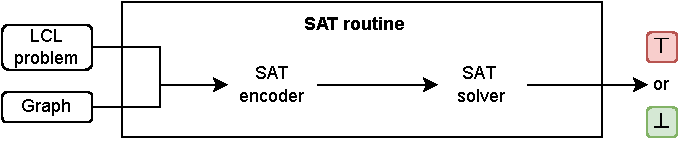
\includegraphics[]{diagrams/implementation_idea_diagram2a.pdf}
\caption{The SAT routine. When given a multigraph and an LCL problem, it checks if a valid labeling exists.}
\label{fig:implementation:1}
\end{figure}

We repeat the routine for each multigraph, as shown in the Algorithm~\ref{alg:counterexample_finder}, and terminate early if the result is $\bot$.
This is illustrated in Figure~\ref{fig:implementation:2}.

\begin{figure}[H]
\centering
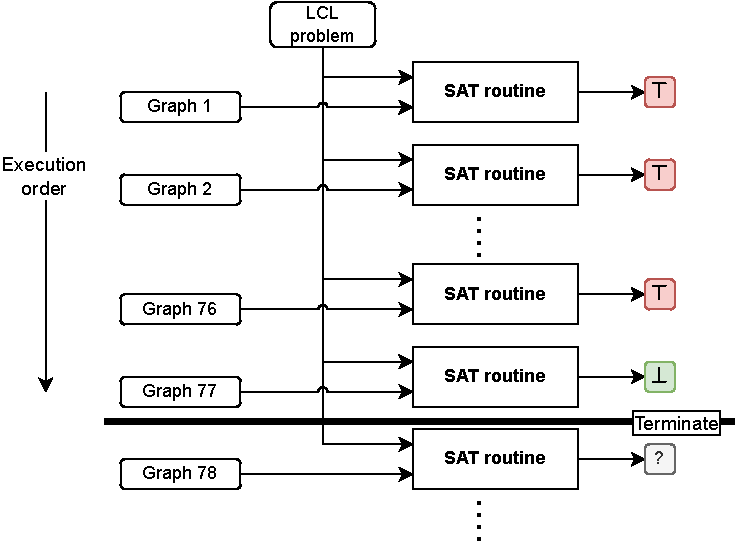
\includegraphics[]{diagrams/implementation_idea_diagram3a.pdf}
\caption{An example of an execution of multiple SAT routines. Execution terminates at the 77th multigraph, when the first unsatisfiable result is encountered.}
\label{fig:implementation:2}
\end{figure}

Now we discuss how we encode an LCL problem $\Pi=(A, P, \Sigma)$ from class $(\Delta, \delta, \lambda)$, and a connected $(\Delta, \delta)$-biregular multigraph $G=(V,E)$, where $V$ is a union of two disjoint sets $V_A$ and $V_P$, into a CNF formula.
Each active node can have possibly any label configuration from $A$ (respectively passive nodes and $P$), and there are always as many ways to arrange the labels of a label configuration as there are permutations of the label configuration.
Let $\operatorname{Perm}(A)$ and $\operatorname{Perm}(P)$ be the sets of all permutations of label configurations in sets $A$ and $P$, respectively.

We define variables $L_{A,u,v,l}$ for each $(u, v)$ incident on an active node $u$ and for each possible label $l \in \Sigma$.
We also define variables $R_{A, u, p}$ for each permutation of label configurations in $A$ and each active node $u$.
Similarly, we define variables $L_{P,u,v,l}$ and $R_{P, u, p}$.

\renewcommand{\labelenumi}{\arabic{enumi}.}
\renewcommand{\labelenumii}{\arabic{enumi}\alph{enumii}.}
We have 3 conditions for our encoding.
Each condition is applied twice, once for active nodes and once for passive nodes.
\begin{enumerate}
\item
  Each node has to agree with their adjacent node on the labels of each edge between them.
  \begin{enumerate}
  \item
    For each $e=(u, v)\in E, u\in V_A$ and each label $(l_1, l_2) \in \Sigma^2, l_1 \neq l_2$, we require that at most one of the variables $L_{A,u,v,l_1}, L_{P,v,u,l_2}$ is true, i.e.\ clause $(\neg L_{A,u,v,l_1} \lor \neg L_{P,v,u,l_2})$.
    \label{enu:sat_conditions:1a}
  \item
    For each $e=(u, v)\in E, u\in V_P$ and each label $(l_1, l_2) \in \Sigma^2, l_1 \neq l_2$, we require that at most one of the variables $L_{P,u,v,l_1}, L_{A,v,u,l_2}$ is true, i.e.\ clause $(\neg L_{P,u,v,l_1} \lor \neg L_{A,v,u,l_2})$
    \label{enu:sat_conditions:1b}
  \end{enumerate}
\item
  Each node can only be applied one permutation of label configurations.
  \begin{enumerate}
  \item
    For an active node $u \in V_A$ and each permutation $p \in \operatorname{Perm}(A)$, we require that only one $R_{A, u, p}$ is true, therefore we add clause $(R_{A, u, p_1} \lor R_{A, u, p_2} \lor \dotsm \lor R_{A, u, p_{|\operatorname{Perm}(A)|}})$ which ensures at least one permutation,
    and clauses
    $ (\neg R_{A, u, p_i} \lor \neg R_{A, u, p_j})$ where $i, j \in \{1, ..., |\operatorname{Perm}(A)|\}, i < j$,
    which ensures at most one permutation.
    We repeat this for each active node $u \in V_A$.
    \label{enu:sat_conditions:2a}
  \item
    For a passive node $u \in V_P$ and each permutation $p \in \operatorname{Perm}(P)$, we require that only one $R_{P, u, p}$ is true, therefore we add clause $(R_{P, u, p_1} \lor R_{P, u, p_2} \lor \dotsm \lor R_{P, u, p_{|\operatorname{Perm}(P)|}})$ which ensures at least one permutation,
    and clauses
    $ (\neg R_{P, u, p_i} \lor \neg R_{P, u, p_j})$ where $i, j \in \{1, ..., |\operatorname{Perm}(P)|\}, i < j$,
    which ensures at most one permutation.
    We repeat this for each passive node $u \in V_P$.
    \label{enu:sat_conditions:2b}
  \end{enumerate}
\item
  A permutation of label configurations implies that a node labels its incident edges according to the permutation.
  \begin{enumerate}
  \item
    For an active node $u \in V_A$, each permutation $p \in \operatorname{Perm}(A)$, and each label $l_i \in p, 1 \leq i \leq \Delta$, we require that $R_{A, u, p}$ implies $L_{A,u,v_i,l_i}$, where $v_i$ is the $i$-th adjacent passive node of active node $u$.
    Therefore, we add clause $(\neg R_{A, u, p} \lor L_{A,u,v_i,l_i})$.
    We repeat this requirement for each active node $u \in V_A$.
    \label{enu:sat_conditions:3a}
  \item
    For a passive node $u \in V_P$, each permutation $p \in \operatorname{Perm}(P)$, and each label $l_i \in p, 1 \leq i \leq \delta$, we require that $R_{P, u, p}$ implies $L_{P,u,v_i,l_i}$, where $v_i$ is the $i$-th adjacent active node of passive node $u$.
    Therefore, we add clause $(\neg R_{P, u, p} \lor L_{P,u,v_i,l_i})$.
    We repeat this requirement for each passive node $u \in V_P$.
    \label{enu:sat_conditions:3b}
  \end{enumerate}
\end{enumerate}

Based on the above conditions and clauses, we encode a CNF by forming a conjunction of clauses.
Formatting the problem as DIMACS CNF can be done with a simple mapping from the variables to unique positive integers, or negative integers in case of a negated variable.
It is quite trivial, therefore we do not discuss more about it.
After obtaining the DIMACS CNF, we feed it into a SAT solver, as showed in Figure~\ref{fig:implementation:1}.
In our implementation, we use the SAT solver called Kissat~\cite{BiereFazekasFleuryHeisinger-SAT-Competition-2020-solvers, Kissat}, which is the winner in the main track of the SAT Competition 2020~\cite{SatCompetition2020}.


\subsection{Generating LCL Problems} \label{sec:implementation:generating_lcl_problems}

We generate a class of LCL problems for a triple $(\Delta, \delta, \lambda)$, where $\Delta$ and $\delta$ are the sizes of label configurations in $A$ and $P$, respectively, and $\lambda$ is the size of $\Sigma$ i.e.\ the number of labels.

The set of all possible label configurations is a $k$-combination with repetitions, where $k$ is the size of a label configuration.
Let $\operatorname{comb}(k, \Sigma)$ be the function that represents $k$-combination with repetitions.
For example, if $\Delta$ is 2, $\Sigma=\{\mathrm{A, B}\}$ and $\lambda$ is 2, then the set of all possible label configurations is
$$ \operatorname{comb}(\Delta, \Sigma) = \{ \{\mathrm{A, A}\}, \{\mathrm{A, B}\}, \{\mathrm{B, B}\} \}. $$

The set of all possible sets of label configurations is a power set of the set of all possible label configurations, excluding an empty set.
Let us define this power set without an empty sets as a function $\operatorname{pow}(d, S)$, where $d$ is the size of a label configuration, and $S$ is the set of all possible label configurations.
For example, the power set of the above example excluding an empty set is
\begin{align*}
  \operatorname{pow}(\Delta, \operatorname{comb}(\Delta, \Sigma)) =  \{&\{\{\mathrm{A, A}\}\}, \\
    &\{\{\mathrm{A, B}\}\}, \\
    &\{\{\mathrm{B, B}\}\}, \\
    &\{\{\mathrm{A, A}\}, \{\mathrm{A, B}\}\}, \\
    &\{\{\mathrm{A, A}\}, \{\mathrm{B, B}\}\}, \\
    &\{\{\mathrm{A, B}\}, \{\mathrm{B, B}\}\}, \\
    &\{\{\mathrm{A, A}\}, \{\mathrm{A, B}\}, \{\mathrm{B, B}\}\} \}.
\end{align*}

The set of all LCL problems of class $(\Delta, \delta, \lambda)$ is defined as
$$ \operatorname{comb}(\Delta, \Sigma) \times \operatorname{comb}(\delta, \Sigma),$$
where $\Sigma$ is any set of labels of length $\lambda$.
%In our implementation, we use the upper-case alphabet as $\Sigma$.
The elements are pairs $(A, P)$, where $A$ is the set of all allowed label configurations for active nodes, and $P$ is the set of all allowed label configurations for passive nodes.

Now that we know how to generate a class of LCL problems, we show the number of problems in classes in Table~\ref{tbl:lcl_problem_classes}.
In the table, we also show the numbers of \emph{purged} and \emph{normalized} problems for each class.
These are the optimizations that reduce the size of problems we have to process through in our implementation, and we discuss them next.

\begin{table}[H]
  \centering
  \begin{tabular}{rrrrrr}
    \toprule
    $\Delta$ & $\delta$ & $\lambda$ & Problems & Purged problems & Purged and normalized problems\\
    \midrule
    1 & 1 & 1 & 1 & 1 & 1 \\
    \midrule
    1 & 1 & 2 & 9 & 3 & 2 \\
    2 & 1 & 2 & 21 & 7 & 5 \\
    2 & 2 & 2 & 49 & 27 & 18 \\
    3 & 2 & 2 & 105 & 67 & 38 \\
    4 & 2 & 2 & 217 & 147 & 84 \\
    4 & 3 & 2 & 465 & 379 & 200 \\
    4 & 4 & 2 & 961 & 843 & 446 \\
    6 & 6 & 2 & 16129 & 15627 & 7926 \\
    \midrule
    2 & 2 & 3 & 3969 & 2103 & 419 \\
    3 & 2 & 3 & 64449 & 44343 & 7735 \\
    3 & 3 & 3 & 1046529 & 962871 & 162299 \\
    %\vdots & \vdots & \vdots & \vdots & \vdots & \vdots\\
    \bottomrule
  \end{tabular}
  \caption{%
    The number of LCL problems in different problem classes.
  }
  \label{tbl:lcl_problem_classes}
\end{table}

Purging is an operation, where an LCL problem is cut down from label configurations that are redundant, in a sense that they cannot possibly be in a valid configuration, no matter what.
These redundant label configurations are found by forming a list of labels that appear in both sets $A$ and $P$.
Then we remove each label configuration from both sets, that have some other labels than what was in the list.

For example, if $A=\{\{\mathrm{A, A}\}, \{\mathrm{A, B}\}, \{\mathrm{B, B}\}\}$ and $P=\{\{\mathrm{A, A}\}, \{\mathrm{A, C}\}, \{\mathrm{C, C}\}\}$, then the labels in $A$ are $\{\mathrm{A, B}\}$ and labels in $P$ are $\{\mathrm{A, C}\}$.
The labels that appear in both $A$ and $P$, i.e.\ $\{\mathrm{A, B}\} \cap \{\mathrm{A, C}\} $ is $\{\mathrm{A}\}$.
Thus, we remove all label configurations from both $A$ and $P$ that contain any other label than $\mathrm{A}$.
In the end, we get $A=\{\{\mathrm{A, A}\}\}$ and $P=\{\{\mathrm{A, A}\}\}$.


Normalizing an LCL problem is an operation of renaming the labels with a permutation such that the resulting problem is the minimum of all permutated problems.
Here, we assume that each label in a label configuration is represented in lexicographic order, and each label configuration is also represented in lexicographic order in both sets $A$ and $P$.
We also assume a common set of labels, the upper-case alphabet.
The total order of two LCL problems is the lexicographic order.
That is, the total order of problems $\Pi_1=(A_1, P_1, \Sigma_1), \Pi_2=(A_2, P_2, \Sigma_2)$ from problem class $(\Delta, \delta, \lambda)$ is $\Pi_1 < \Pi_2$ if and only if $A_1 < A_2$ or $(A_1 = A_2 \text{ and } P_1 < P_2)$.
The result of normalization is an LCL problem in its \emph{canonical form}.
After normalizing any two isomorphic LCL problems, their appearance is identical.

For example, the problems
$$\Pi_1=(\{\{\mathrm{B, B}\}\}, \{\{\mathrm{A, C}\}, \{\mathrm{C,C\}}\}, \Sigma),$$
$$\Pi_2=(\{\{\mathrm{D, D}\}\}, \{\{\mathrm{A,A\}},\{\mathrm{E, A}\}\}, \Sigma),$$ after normalization look like
$$\Pi_1'=(\{\{\mathrm{A, A}\}\}, \{\{\mathrm{B, B}\},\{\mathrm{B, C}\}\}, \Sigma),$$
$$\Pi_2'=(\{\{\mathrm{A, A}\}\}, \{\{\mathrm{B, B}\},\{\mathrm{B, C}\}\}, \Sigma),$$ (denoted by a prime).

In our implementation, we first generate all LCL problems.
Then we use the purge operation for each LCL problem, and remove problems that have an empty set of label configurations.
Finally, we normalize each problem, and remove duplicates.
The amount of problems after purging and normalizing can be seen in Table~\ref{tbl:lcl_problem_classes}.



\subsection{Optimizations} \label{sec:implementation:optimizations}
In this section, we will discuss some optimizations used in the implementation that we have not yet mentioned in previous sections.
The optimizations we discuss here briefly, utilizes either parallelization or caching.

When we generate graphs with \emph{genbg}, we actually do it in parallel.
If we give \emph{genbg} the option \codee{r/m}, it generates the \codee{r}-th subset of \codee{m} roughly equal sized subsets.
For some fixed $m$ we can generate each subset in parallel by giving each option \codee{0/m}, \codee{1/m}, \dots, \codee{m-1/m} to different threads.
This makes it roughly $t$-times faster, where $t$ is the number of threads used, assuming that there are $t$ available cores in the system.

When multigraphs are generated, we can optionally save them into a database.
Then multigraphs can be fetched from the database when needed, nearly for free in terms of time.
Similarly, LCL problems can also be saved into the database, and automatically fetched from there.

In our implementation, finding counterexamples for multiple LCL problems is done in parallel, utilizing all logical cores of the system.
This can be done quite trivially, as different instances of finding counterexamples do not really depend on each other.
They only depend on the multigraphs to generate SAT problems, which can be accessed safely with read-only access.
